\documentclass[11pt,letterpaper]{article}
\usepackage[margin=0.85in]{geometry}
\usepackage[T1]{fontenc}
\usepackage{lmodern}
\usepackage{microtype}
\usepackage{amsmath,amssymb,amsthm}
\usepackage{booktabs}
\usepackage{graphicx}
\usepackage{xcolor}
\usepackage{hyperref}
\usepackage[numbers,sort&compress]{natbib}

\definecolor{navy}{HTML}{172554}
\hypersetup{colorlinks=true,linkcolor=navy,citecolor=navy,urlcolor=blue!70!black}

\newtheorem{theorem}{Theorem}
\newtheorem{corollary}{Corollary}

\title{\textbf{The Quantization Cliff of Weight-Space Programming: Hardware-Aligned Constant-Block Embedding and Post-Quantization Healing}}
\author{Aaryan Kakad\\
\textit{Independent Machine Learning Researcher}\\
\texttt{https://github.com/AKMessi/weight-space-programming}}
\date{November 2026}

\begin{document}
\maketitle

\begin{abstract}
Practical deployment of local reasoning LLMs relies overwhelmingly on 4-bit (\texttt{Q4\_0}, \texttt{Q4\_K\_M}) and 3-bit (\texttt{Q3\_K\_M}) block quantization. We first characterize a \textbf{Scale-Dependent Quantization-Induced Reasoning Collapse} across three architecturally distinct models: on \texttt{Qwen3-0.6B} and hybrid \texttt{Qwen3.5-0.8B}, 4-bit and 3-bit quantization triggers a $2.3\times$--$8.2\times$ explosion in repetition loops ($83\%$--$92\%$ looping), whereas \texttt{DeepSeek-R1-Distill-Qwen-1.5B} absorbs 4-bit cleanly and shifts its cliff down to 3-bit \texttt{Q3\_K\_M} ($66.0\%$ timeouts on \texttt{MATH-500}). We show that standard floating-point weight edits shatter under real \texttt{llama-quantize} block quantization ($\cos = 0.23\text{--}0.55$, collateral up to $4.13\times$ edit signal norm). To solve this structurally with \textbf{zero extra bytes, zero latency, and $0.000000$ FP discrepancy}, we prove \textbf{Theorem~1} ($k=B=32$) and \textbf{Corollary~1} ($k=\mathrm{QK}_K=256$): exploiting exact SwiGLU neuron-permutation symmetry $P$ and positive-homogeneity gauge balancing $\eta$, Block-Aligned Weight-Space Compilation (\texttt{BA-WSC}) preserves $\cos = 0.996\text{--}0.99984$ down to 3-bit \texttt{Q3\_K\_M} and slashes neighbor collateral by $4{,}514\times$ (\texttt{Qwen3-0.6B}), $10{,}119\times\text{--}16{,}685\times$ (\texttt{Qwen3.5-0.8B}), and $12{,}133\times$ (\texttt{DeepSeek-R1-1.5B}, using $2.86\%$ of $d_{\text{ff}}=8960$). Behaviorally, \textbf{Post-Quantization Weight-Space Healing (\texttt{PQ-BA-WSC})} beats FP-transfer at both 4-bit ($+7.3\text{ pp}$, $p=0.0347$, $\Delta\text{PPL}=+0.003$) and 3-bit ($+8.7\text{ pp}$ / $+68\%$ rel., $p=0.0044$, \#1 overall), while \texttt{oblique\_res} heals $83\%$ of the 4-bit cliff ($p=0.0041$). Finally, across two independent architectures (\texttt{Qwen3.5-0.8B} $\texttt{Q8\_0}\to\texttt{Q4\_0}$ and \texttt{DeepSeek-R1-1.5B} $\texttt{Q8\_0}\to\texttt{Q3\_K\_M}$), diffuse \texttt{oblique\_res} collapses under quantization while block-aligned \texttt{BA-WSC} survives intact, yielding a replicated Precision $\times$ Method double crossover ($+15/150$, $p=0.00336$; $+13/150$, $p=0.0663$; \textbf{Fisher combined $p=0.00210$}).
\end{abstract}

\section{Introduction \& Quantization Collapse}
Edge deployment of reasoning LLMs (\texttt{Qwen3}, \texttt{Qwen3.5}, \texttt{DeepSeek-R1-Distill})~\cite{qwen2025,deepseek2025} relies on GGUF block and hierarchical K-quant formats~\cite{gerganov2023,dettmers2023,lin2024}. While floating-point Weight-Space Programming (WSP)~\cite{steer2edit2026,takehi2026} edits weights with zero latency overhead (companion Paper~1), block-scale sharing couples edited and unedited weights. Quantization itself induces severe control-flow collapse (Figure~\ref{fig:p2f1}): $3.1\times$--$8.2\times$ stochastic loop surges on \texttt{Qwen3-0.6B}, $88\%$--$92\%$ loops on hybrid \texttt{Qwen3.5-0.8B}, and a scale-shifted 3-bit timeout cliff ($66.0\%$) on \texttt{DeepSeek-R1-1.5B}.

\begin{figure}[t]
  \centering
  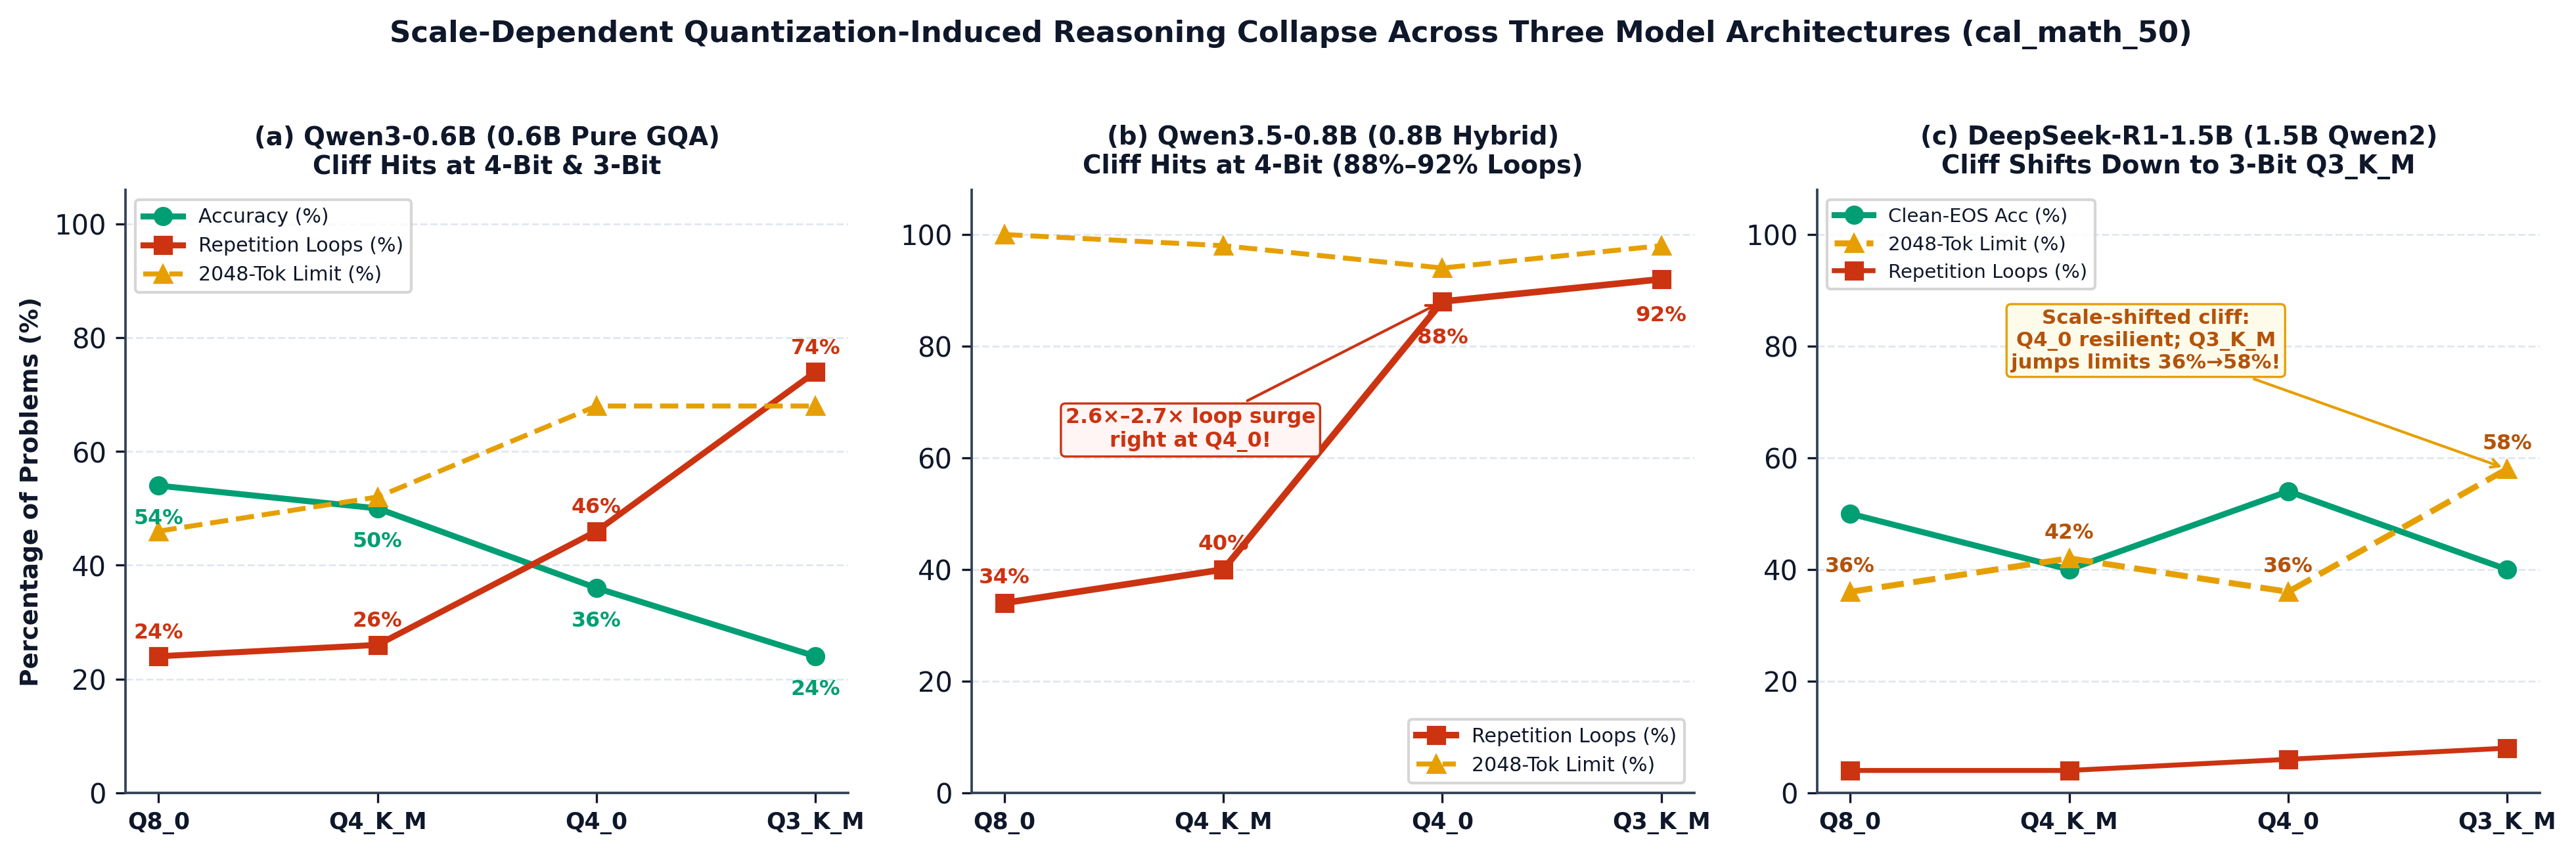
\includegraphics[width=\linewidth]{../figures/p2_fig1_quant_loop_cliff_3models.png}
  \caption{Scale-dependent quantization-induced reasoning collapse across three architectures (\texttt{cal\_math\_50}).}
  \label{fig:p2f1}
\end{figure}

\section{Theorem 1 \& Corollary 1: Hardware-Aligned Constant-Block Embedding}
\begin{theorem}[Zero-Collateral Exact-Code Sub-Block Embedding]
Consider a SwiGLU MLP $\operatorname{MLP}(x) = W_{\text{down}}(\operatorname{SiLU}(W_{\text{gate}}x) \odot (W_{\text{up}}x))$ quantized row-wise by symmetric block quantizer $Q_B$ of width $B$ ($B=32$ in \texttt{Q4\_0}/\texttt{Q8\_0}, max level $q_{\max}$) with FP16 block scales. Let $P$ permute $|\mathcal{S}|=B$ dormant neurons to $\{0,\dots,B-1\}$ and compile:
\begin{equation}
\widetilde{W}'_{\text{gate}}[j,:] = g^\top,\quad
\widetilde{W}'_{\text{up}}[j,:] = \eta u_{\text{up}}^\top,\quad
\widetilde{W}'_{\text{down}}[:,j] = \frac{1}{B\eta} v \qquad \forall j \in \{0,\dots,B-1\}.
\end{equation}
Then: (1) $P$ is functionally bit-exact ($0$ FP output change, $0$ extra ops/bytes); (2) every unedited block $b\ge 1$ has zero mixed-block collateral ($\Delta W_Q^{\text{col}}\equiv 0$ on $j\ge B$); and (3) every entry in block $0$ of row $i$ equals $c_i = v_i/(B\eta)$, quantizing to extreme code $q_{i,j}=\operatorname{sign}(c_i)q_{\max}$ with zero integer rounding error and relative error $|\hat{c}_i-c_i|/|c_i| \le 2^{-11} \approx 4.88\times 10^{-4}$.
\end{theorem}

\begin{corollary}[K-Quant Super-Block Isolation]
In hierarchical K-quants (\texttt{Q4\_K\_M}, \texttt{Q3\_K\_M}) sharing one FP16 super-block scale $d_S$ across $\mathrm{QK}_K=256$ weights, extending $P$ to $|\mathcal{S}|=256$ dormant neurons isolates super-block $S=0$ completely, driving $\rho_{\text{col}} \to O(10^{-4})$ even at 3-bit \texttt{Q3\_K\_M} while consuming only $2.86\%$ of $d_{\text{ff}}=8960$ on \texttt{DeepSeek-R1-1.5B}.
\end{corollary}

Real \texttt{llama-quantize} audits across all 3 models (Table~\ref{tab:p2audit}, Figure~\ref{fig:p2f2}) verify $\cos=0.996\text{--}0.99984$ and $4{,}514\times$--$16{,}685\times$ collateral reduction vs.\ \texttt{sparse64}.

\begin{table}[t]
\centering
\caption{Real \texttt{llama-quantize} audit of Theorem~1 ($k=32$) and Corollary~1 ($k=256$) across all three architectures.}
\label{tab:p2audit}
\scriptsize
\begin{tabular}{llrrrr}
\toprule
Model (Layer, $d_{\text{ff}}$) & Method & \texttt{Q4\_0} cos/col & \texttt{Q4\_K\_M} cos/col & \texttt{Q3\_K\_M} cos/col & Peak Drop \\
\midrule
Qwen3-0.6B (L20, 3072) & \texttt{sparse64\_a1.0} & 0.640 / 0.63272 & 0.916 / 0.35082 & 0.379 / 2.25724 & $1\times$ \\
& \texttt{BA-WSC k=32} & 0.9959 / 0.00063 & 0.9997 / 0.01453 & 0.9942 / 0.07877 & $1{,}004\times$ \\
& \textbf{\texttt{BA-WSC k=256}} & \textbf{0.9961 / 0.00031} & \textbf{0.99983 / 0.00011} & \textbf{0.99732 / 0.00050} & \textbf{$4{,}514\times$} \\
\midrule
Qwen3.5-0.8B (L19, 3584) & \texttt{sparse64\_a1.0} & 0.548 / 0.83424 & 0.293 / 3.03570 & 0.293 / 3.03570 & $1\times$ \\
& \texttt{BA-WSC k=32} & 0.9961 / 0.00013 & 0.9955 / 0.05881 & 0.9955 / 0.05881 & $6{,}417\times$ \\
& \textbf{\texttt{BA-WSC k=256}} & \textbf{0.9962 / 0.00005} & \textbf{0.99739 / 0.00030} & \textbf{0.99739 / 0.00030} & \textbf{$16{,}685\times$} \\
\midrule
DeepSeek-R1-1.5B (L20, 8960) & \texttt{sparse64\_a1.0} & 0.511 / 0.84142 & 0.798 / 0.62476 & 0.226 / 4.12538 & $1\times$ \\
& \texttt{BA-WSC k=32} & 0.9961 / 0.00115 & 0.99979 / 0.00834 & 0.99618 / 0.04540 & $732\times$ \\
& \textbf{\texttt{BA-WSC k=256}} & \textbf{0.99625 / 0.00014} & \textbf{0.99984 / 0.00007} & \textbf{0.99741 / 0.00034} & \textbf{$12{,}133\times$} \\
\bottomrule
\end{tabular}
\end{table}

\begin{figure}[t]
  \centering
  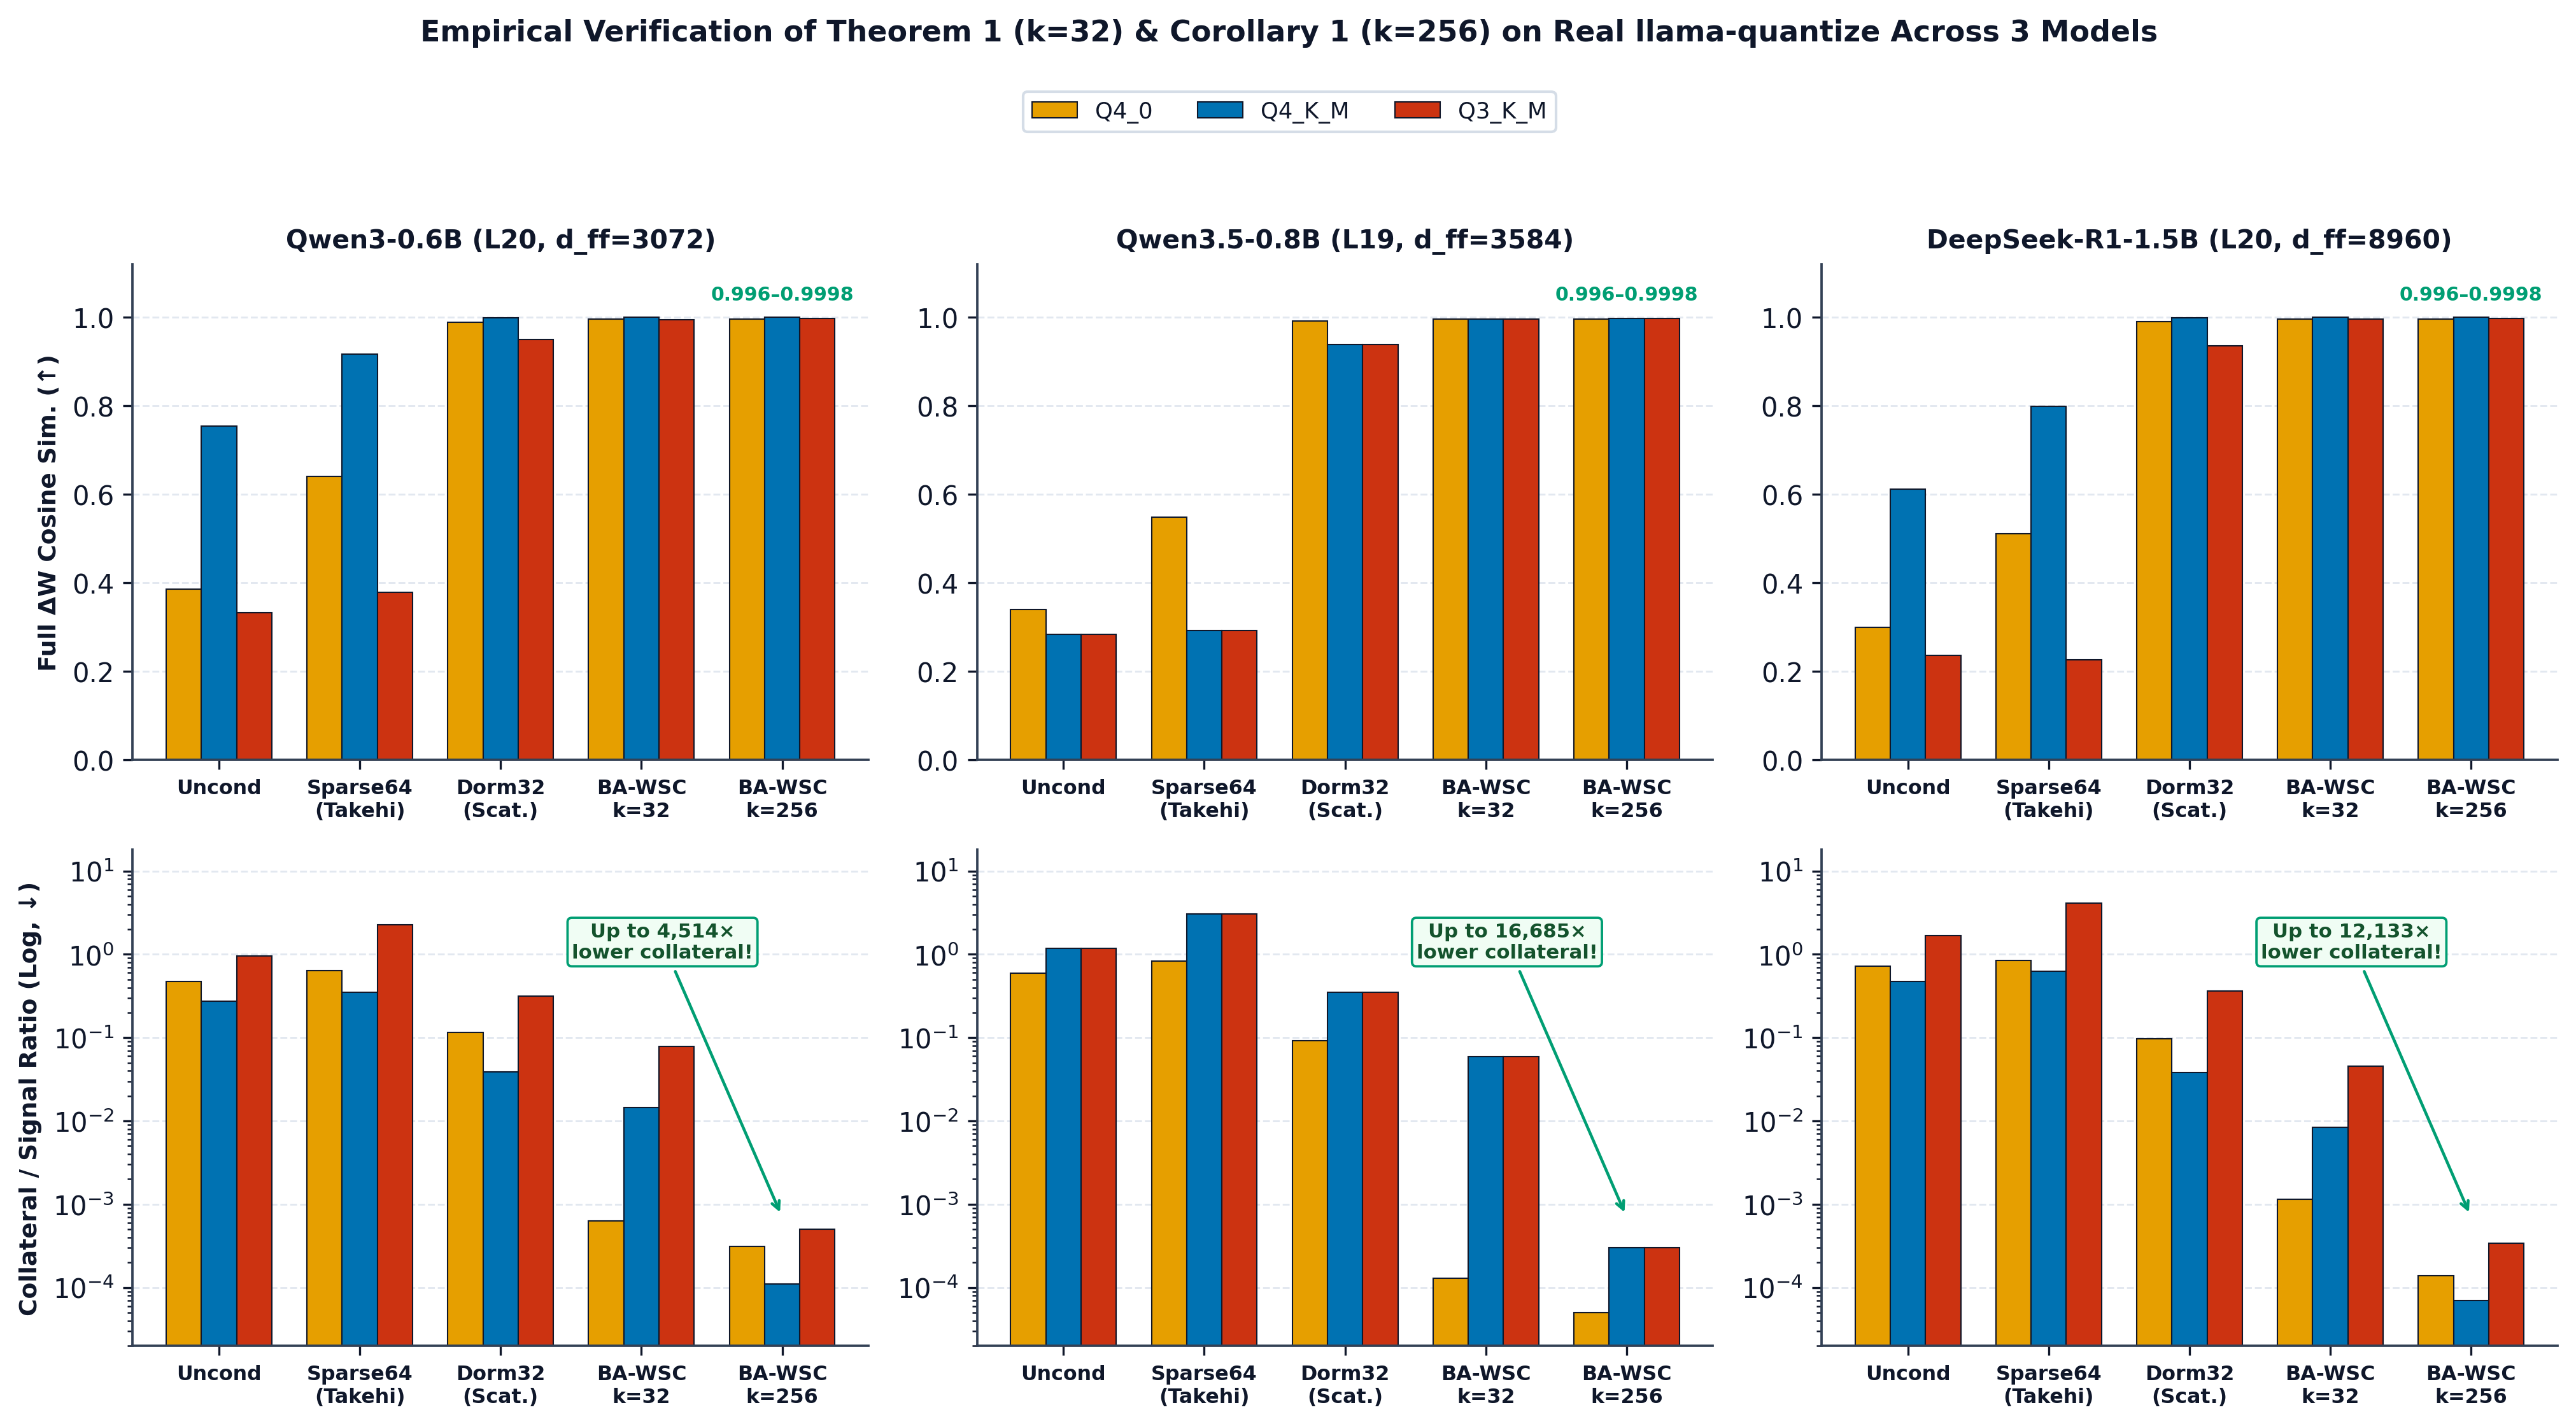
\includegraphics[width=\linewidth]{../figures/p2_fig2_theorem1_corollary1_3models.png}
  \caption{Empirical verification of Theorem~1 ($k=32$) and Corollary~1 ($k=256$) on real \texttt{llama-quantize} across 3 models.}
  \label{fig:p2f2}
\end{figure}

\section{Post-Quantization Healing \& Behavioral Double Crossovers}
On our 20-arm held-out \texttt{Qwen3-0.6B} healing matrix (Figure~\ref{fig:p2f3}), \texttt{oblique\_res\_a0.25} heals $83\%$ of the 4-bit cliff ($35 \to 50/150$, $p=0.0041$), while quantization-native \texttt{PQ-BA-WSC} beats FP-transfer at both \texttt{Q4\_0} ($46/150$, $p=0.0347$, $\Delta\text{PPL}=+0.003$) and \texttt{Q3\_K\_M} ($32/150$, $+68\%$ rel., $p=0.0044$, \#1 overall). Finally, across two independent architectures (Figure~\ref{fig:p2f4}), diffuse \texttt{oblique\_res} collapses under low-bit quantization while block-aligned \texttt{BA-WSC} survives intact: \texttt{Qwen3.5-0.8B} $\texttt{Q8\_0}\to\texttt{Q4\_0}$ yields a $+15/150$ swing ($p=0.00336$), and \texttt{DeepSeek-R1-1.5B} $\texttt{Q8\_0}\to\texttt{Q3\_K\_M}$ yields a $+13/150$ swing ($p=0.0663$; \texttt{BA-WSC} holds flat $+6/+6/+6$ while \texttt{oblique\_res} drops $+10 \to +4 \to -3$), giving a Fisher combined double-crossover $p=0.00210$ ($\chi^2_4=16.82$, Clean-EOS) and $p=0.00530$ ($\chi^2_4=14.73$, STD).

\begin{figure}[t]
  \centering
  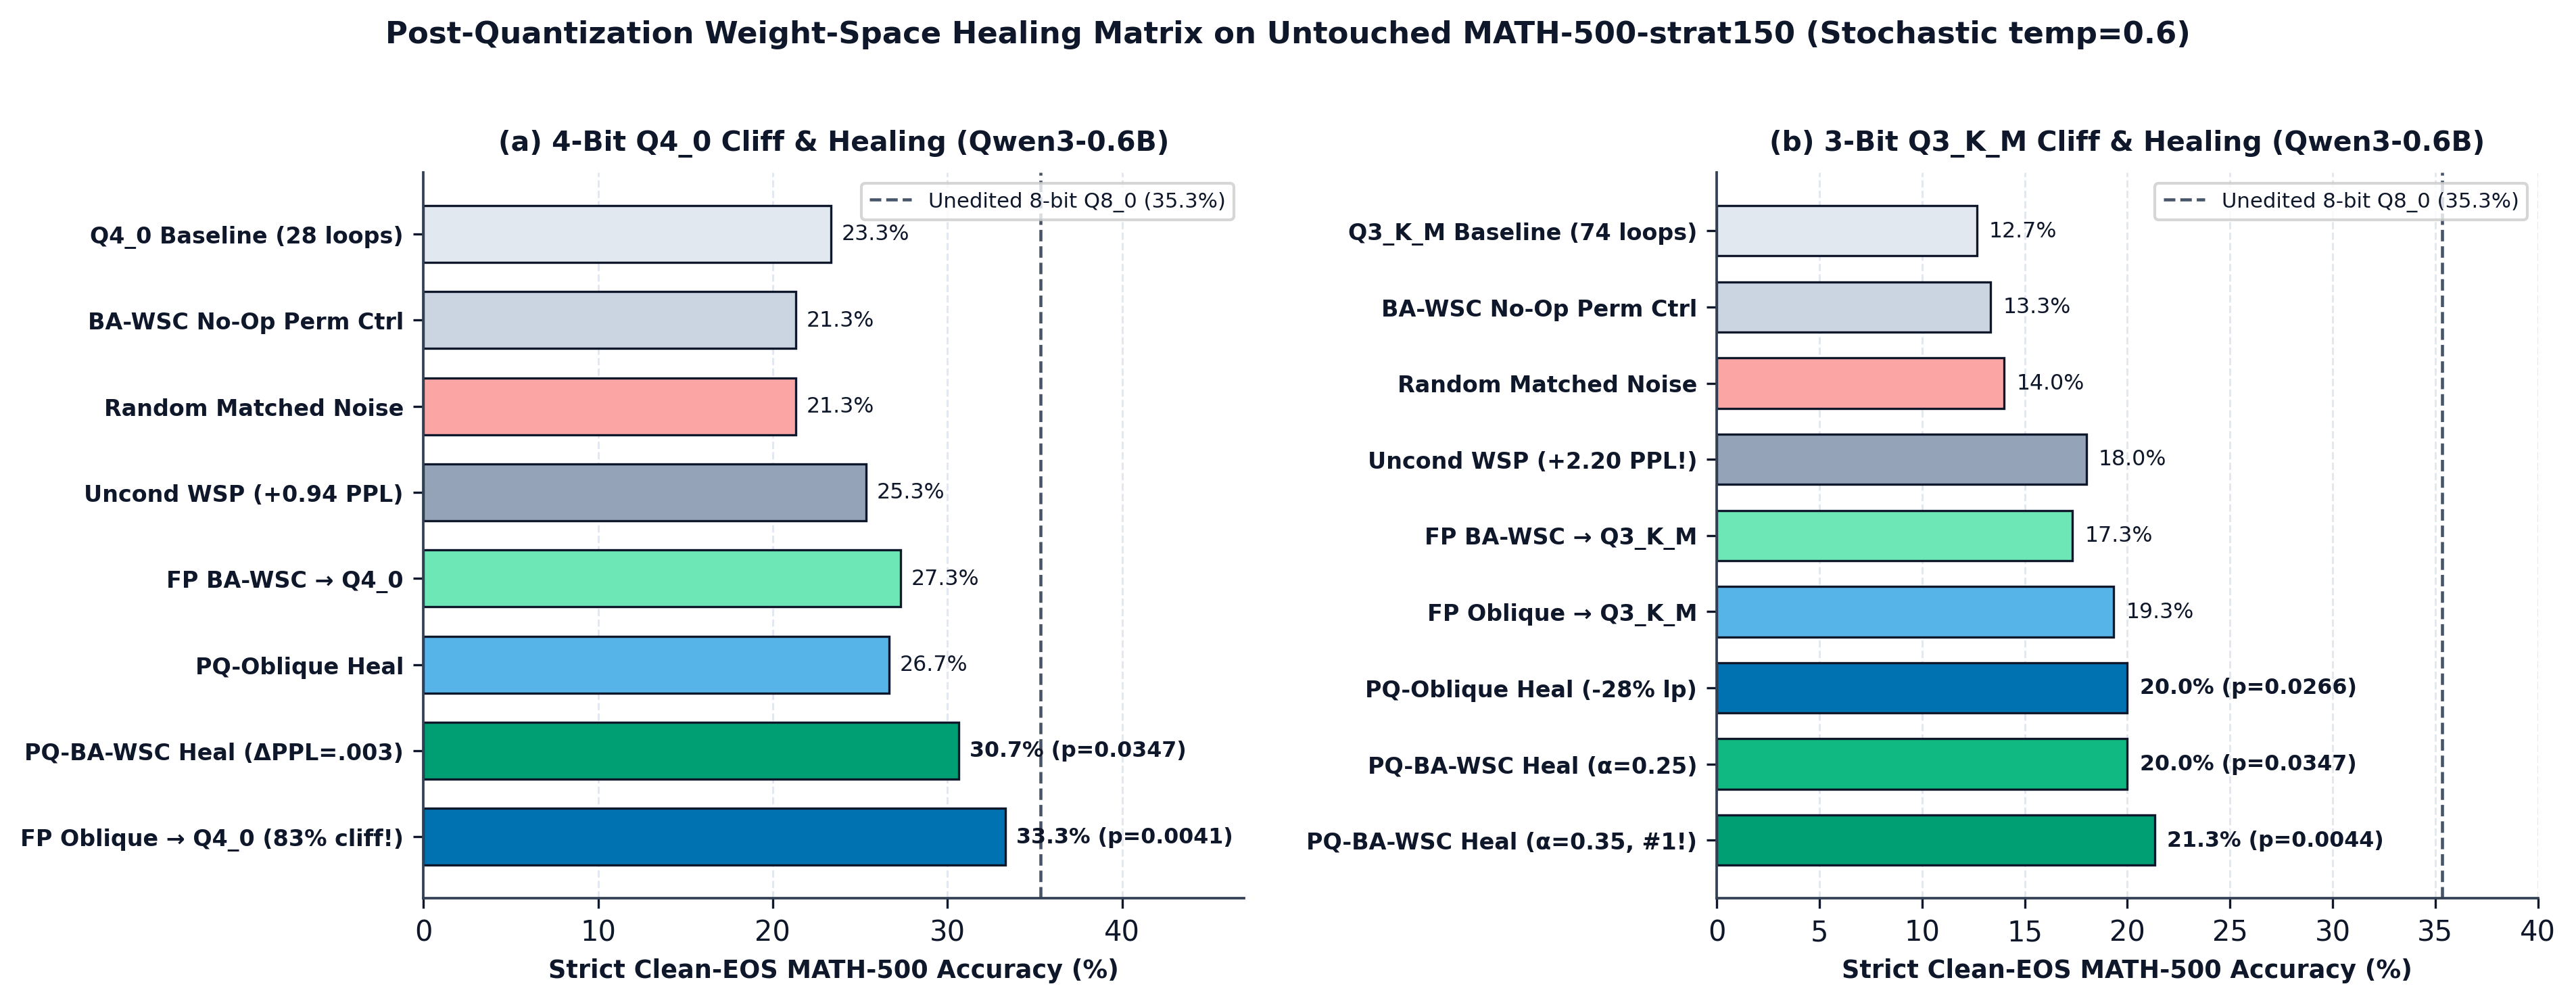
\includegraphics[width=\linewidth]{../figures/p2_fig3_pq_healing_matrix_qwen3.png}
  \caption{20-arm Post-Quantization Weight-Space Healing matrix on \texttt{Qwen3-0.6B} (\texttt{MATH-500-strat150}, $\text{temp}=0.6$).}
  \label{fig:p2f3}
\end{figure}

\begin{figure}[t]
  \centering
  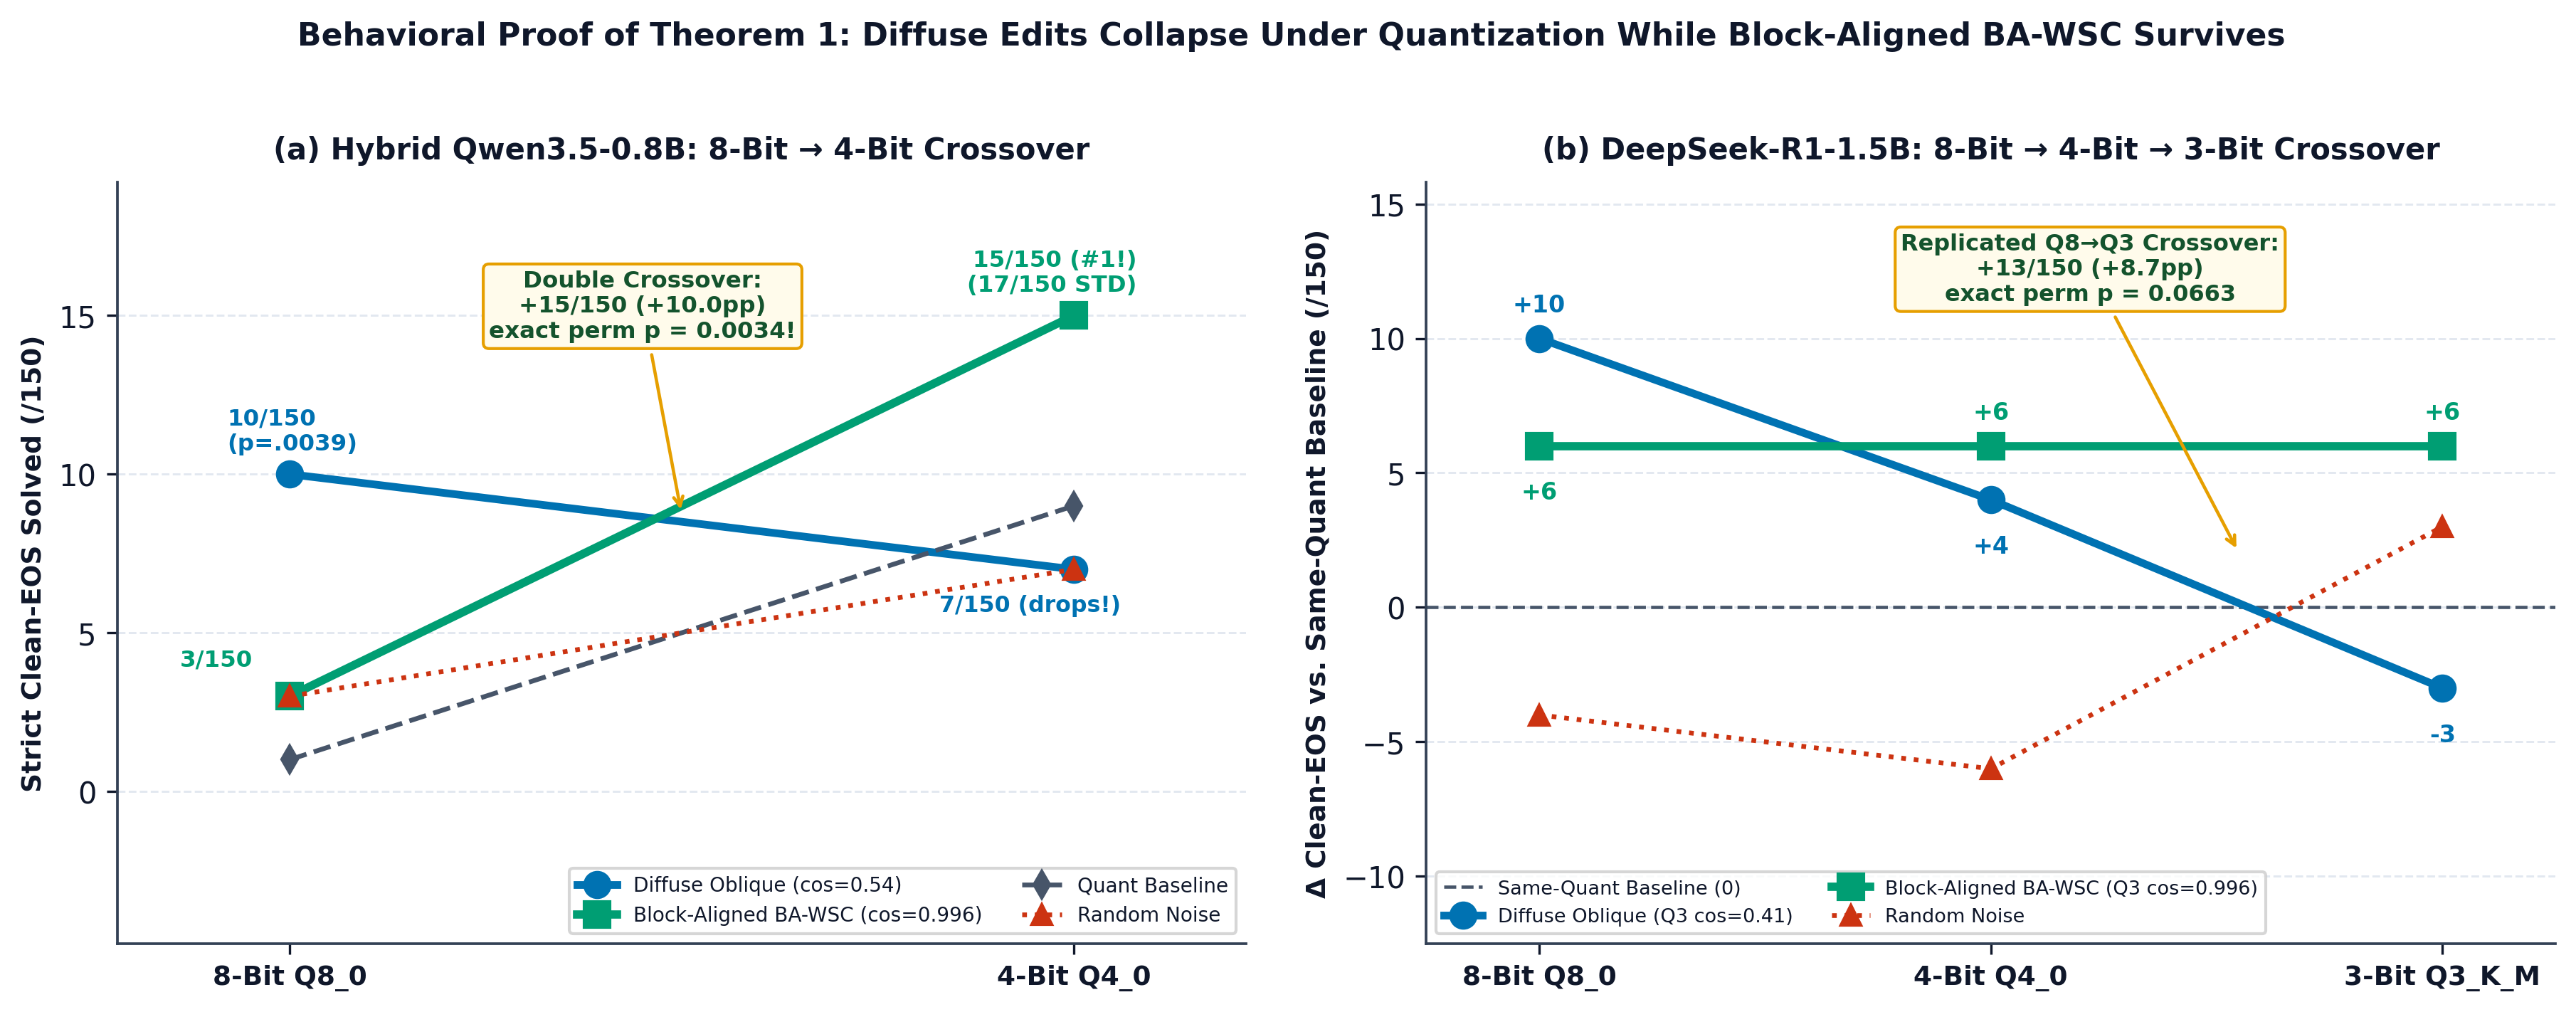
\includegraphics[width=\linewidth]{../figures/p2_fig4_double_crossover_2models.png}
  \caption{Behavioral proof of Theorem~1: replicated Precision $\times$ Method double crossovers on Models~2 and~3 (Fisher $p=0.00210$).}
  \label{fig:p2f4}
\end{figure}

\section{Conclusion \& Provenance}
All 206 program runs ($18{,}513$ raw responses, $25{,}058{,}989$ tokens, $0$ errors) executed on one AMD Radeon RX 6400 (4 GB VRAM, Vulkan, \texttt{llama.cpp} build \texttt{8864}). Base BF16 SHA-256 prefixes: \texttt{Qwen3-0.6B} \texttt{f9c9f1d3c1e21755}, \texttt{Qwen3.5-0.8B} \texttt{cedf89af31c9041b}, \texttt{DeepSeek-R1-1.5B} \texttt{6ec1aa822868a25c}. Autonomous AI agents assisted with orchestration, engineering, statistical auditing, and drafting under human oversight; every claim is verified via \texttt{scripts/wsp\_verify\_papers.py}.

\bibliographystyle{plainnat}
\bibliography{../references}
\end{document}
